\documentclass[11pt]{beamer}
\usetheme{Warsaw}
\usepackage[utf8]{inputenc}
\usepackage[brazil]{babel}  % idioma
\usepackage{amsmath,amsfonts,amssymb,textcomp}
\usepackage{graphicx}
\usepackage{subfigure}

\author{Othon Oliveira}
\title{Sistemas Operacionais}
%\setbeamercovered{transparent} 
%\setbeamertemplate{navigation symbols}{} 
%\logo{} 
\institute{Fatec -- Faculdade de Informática --- PE} 
\date{15-Fev-2016} 
%\subject{} 
\begin{document}


% Capa - requer o TikZ
\newcommand{\capa}{
    \begin{tikzpicture}[remember picture,overlay]
        \node at (current page.south west)
            {\begin{tikzpicture}[remember picture, overlay]
                \fill[shading=radial,top color=orange,bottom color=orange,middle color=yellow] (0,0) rectangle (\paperwidth,\paperheight);
            \end{tikzpicture}
          };
    \end{tikzpicture}
}


\begin{frame}
\titlepage
\end{frame}

%\begin{frame}
%\tableofcontents
%\end{frame}



%+++++++++++++++++++++++++++++++++++++++++++++++
\begin{frame}{Exemplos de sistemas operacionais}
\begin{figure}[h]
%\left

\includegraphics[width=18mm, height=15mm]{Figuras/appleOficial.jpg}
\qquad \quad \quad \quad \quad

\includegraphics[width=19mm, height=17mm]{Figuras/windows.png}
\qquad \quad \quad \quad \quad \quad \quad 	\vspace{1.0in}
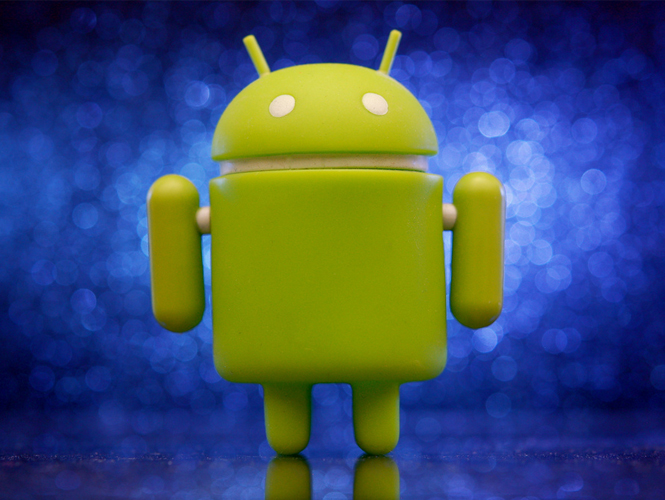
\includegraphics[width=15mm, height=15mm]{Figuras/android.jpg}
\qquad \quad \quad \quad \quad \quad \quad \quad 

\includegraphics[width=25mm, height=15mm]{Figuras/ubuntu_904.jpg}

\end{figure}
\end{frame}

%+++++++++++++++++++++++++++++++++++++++++++++++
\begin{frame}{Funções de um S.O.}
  \begin{itemize}
  \item gerência de processos *
  \item gerência de memória
  \item sistema de gerência de arquivos \textit{filesystem}
  \item gerência de entrada e saída
  \end{itemize}
\end{frame}


%+++++++++++++++++++++++++++++++++++++++++++++++
\begin{frame}{História}
  Evolução: Os S.O. vêm passando por um processo intenso de evolução.
	
  \vspace{0.2in}
	
  Computação digital: O primeiro computador DIGITAL foi projetado pelo matemático Charles Babbage(1792 -- 1871).
  Babbage empregou grande parte da sua fortuna para construir sua 'máquina analítica', porém nunca conseguiu vê-la funcionando
  de modo apropriado, pois era mecânico e a tecnologia da sua época não era capaz de produzir as engrenagens e correias de precisão 
  que eram necessárias.
  Babbage percebeu que seria preciso um software para sua máquina analítica. \\
  Pergunta: Seria um sistema operacional ??
\end{frame}

%+++++++++++++++++++++++++++++++++++++++++++++++
\begin{frame}{História}
	1ª geração (1945 -- 1955): Válvulas e Painéis de programação.
	Após os infrutíferos fracassos até a 2ª guerra mundial, destacamos a arquitetura de J. Von Neumann

	\begin{figure}[h]
	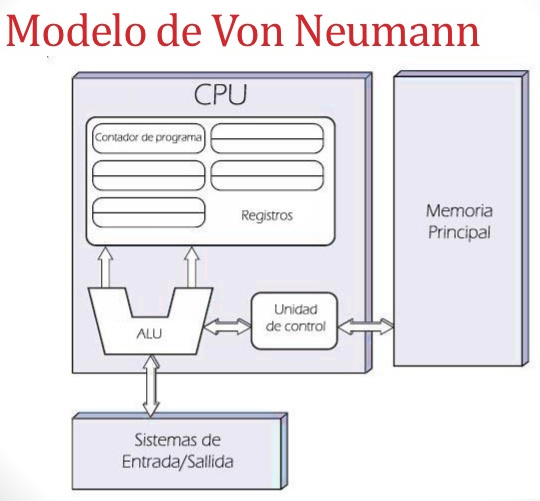
\includegraphics[width=60mm, height=40mm]{Figuras/modelo-de-von-neumann.jpg}
	\end{figure}

\end{frame}


%+++++++++++++++++++++++++++++++++++++++++++++++
\begin{frame}{História, continuação}
	2ª geração (1955 -- 1965) Transistores e sistemas em lote (batch)
	\vspace{0.2in}
  \begin{itemize}
	    \item Os computadores tornaram-se suficientemente confiáveis.
	    \item Comercialização de alguns computadores que funcionavam por um tempo útil a fim de executar uma tarefa por completo.
	    \item Conhecidos por ``mainframe'' ou computadores de grande porte, ex: IBM /360, IBM /370
	    \item Ocupavam grandes salas e até prédios inteiros para um único computador.
  \end{itemize}	
Um JOB (um ou conjunto de programas) era feito em cartões perfurados. 
Esses cartões eram levados à sala de entradas e entregues a um operador, após algum tempo retornava para levar a saída impressa. 
O Operador executava esses Jobs, gerava arquivos de saída que eram levados à sala de impressão.
\end{frame}



%+++++++++++++++++++++++++++++++++++++++++++++++
\begin{frame}{História -- 2ª geração}
	\begin{figure}[h]
	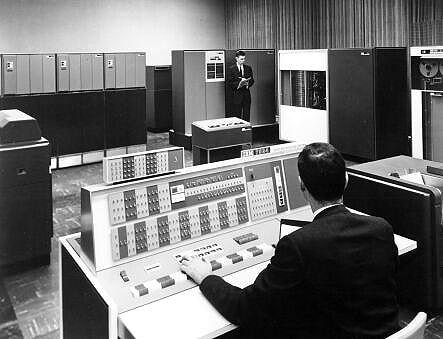
\includegraphics[width=60mm, height=40mm]{Figuras/2-geracao.jpg}
	\end{figure}

\end{frame}

%+++++++++++++++++++++++++++++++++++++++++++++++
\begin{frame}{História}
  3ª geração (1965 -- 1980) CIs e multiprogramação
  \vspace{0.2in}
  
  Existiam dois tipos de computadores distintos e incompatíveis, no início da década de 60'.
  Os científicos, orientados como o 7094 -- para cálculos científicos e para engenharia.
  Os comerciais, orientados a caracteres como o 1401 muito utilizado em bancos, cia de seguros e governos.
  A IBM torna-se a primeira grande CIA fabricantes que conseguiu alguma compatibilidade, ex: /360
  Nessa geração o conceito de multiprogramação foi criado. Antes, até que uma tarefa fosse executada, os dispositivos (E/S, CPU) ficavam parados.
  Solução: dividir a memória em várias partes, com um job diferente em cada partição. Enquanto um JOB esperava que a operação de E/S terminasse
  outro JOB poderia estar ocupando a CPU, logo ela não ficava ociosa a maior parte do tempo.
\end{frame}


%+++++++++++++++++++++++++++++++++++++++++++++++

\begin{frame}{História}
  4ª geração (1980 -- 1990) Computadores pessoais.\\
  \vspace{0.2in}
  Com o desenvolvimento dos computadores em larga escala, \textit{large scale integration -- LSI}, os chips são integrados em grandes quantidades
  numa única pastilha -- \textit{waffle}.\\
  A Intel lançou o 8080 -- primeira CPU de 8 bits de propósito geral, mas não tinha um S.O.
  Alguns Exemplos de PCs: CP/M, IBM PC, DOS, MS-DOS, ...
  
\end{frame}


%+++++++++++++++++++++++++++++++++++++++++++++++

\begin{frame}{História}
  5ª geração (1990 -- atual) Smartphones, Tablets, ...\\
  \vspace{0.2in}
  Curiosamente esses equipamentos não utilizam as CPU da Intel(AMD) ou arquitetura CISC, Pipelines muito complicados.
  A maioria dos Smartphones, Tablets têm CPU ARM (da Texas?), utilizam arquitetura RISC uso intenso de Pipelines.  
  
\end{frame}




\begin{frame}{Pesquisa: O Zoológico de Sistemas Operacionais}
 \begin{itemize}
  \item S.O. de computadores de grande porte;
  \item S.O. servidores;
  \item S.O. de multiprocessadores;
  \item S.O. de computadores pessoais;
  \item S.O. de tempo real -- ou tempo crítico;
  \item S.O. embarcados;
  \item S.O. de cartões inteligentes.
 \end{itemize}
 
\end{frame}

%+++++++++++++++++++++++++++++++++++++++++++++++

\begin{frame}{Pesquisa: Estruturas de um sistema de computação}
 \begin{itemize}
  \item S.O. Monolíticos (a mais comum);
  \item S.O. de camadas (ex: Sistema MULTICS);
  \item S.O. de máquinas virtuais;
  \item S.O. de exonúcleos (VM /370 -- cada partição tem uma cópia exata do computador real);
  \item S.O. Cliente -- Servidor.
 \end{itemize}
 
\end{frame}

%+++++++++++++++++++++++++++++++++++++++++++++++


\begin{frame}{Vídeo}
 Apagar as luzes, por favor !!!
\end{frame}



\end{document}
